% Document setup
%-----------------------------------------------------------------------------%
\documentclass[11pt]{article}
\usepackage[a4paper, margin=1.5cm]{geometry}
\raggedright
\usepackage[parfill]{parskip}
\usepackage{graphicx}
\usepackage{siunitx}
%-----------------------------------------------------------------------------%
% Import packages
%-----------------------------------------------------------------------------%
\usepackage{amsmath}
%-----------------------------------------------------------------------------%

% The document itself
%-----------------------------------------------------------------------------%
\begin{document}
%-----------------------------------------------------------------------------%
\section{DC Motor Circuit}
As an electrical schematic a DC motor can be represented as:
\begin{figure}[h]
  \centering
  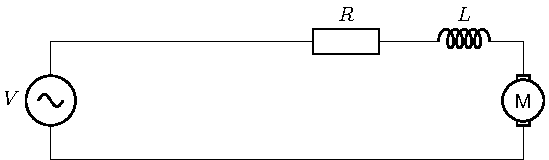
\includegraphics{motor_schematic/motor_schematic.pdf}
  \caption{Electrical diagram of DC motor.}
\end{figure}

By introducing an armature constant of the motor $K_t$, the torque the motor produces, $T$, is related to the armature current of the motor by:
\begin{equation}
  T = K_t i
\end{equation}

Similarly the motor back emf, $e$, is related to the rotational speed, $\dot{\theta}$ using the motor constant $K_e$ by:
\begin{equation}
  e = K_e \dot{\theta}
\end{equation}

From Kirchhoff's law the sum of potential differences in a closed loop must be zero. This leads to:
\begin{equation}
  iR + \frac{di}{dt}L = V - k_e\dot{\theta}
\end{equation}

\section{Inertia}
The inertia of the motor armature must also be considered.
From Newton's second law:
\begin{equation}
  J\ddot{\theta} + B\dot{\theta} = T
\end{equation}

Where $J$ is the motor inertial constant, and $B$ the motor damping constant.

\section{State-space Equations}
The following equations:
\begin{subequations}
  \begin{align}
    iR + \frac{di}{dt}L &= V - k_e\dot{\theta} \\
    J\ddot{\theta} + B\dot{\theta} &= T
  \end{align}
\end{subequations}

can be written in state-space form.
Selecting $\dot{\theta}$, $\ddot{\theta}$ and $i$ as the state variables:
\begin{equation}
  \dot{\theta} = \dot{\theta}
\end{equation}

For the inertia:
\begin{subequations}
  \begin{align}
    J\ddot{\theta} + B\dot{\theta} &= T \\
    \ddot{\theta} + \frac{B}{J}\dot{\theta} &= \frac{T}{J} \\
    \ddot{\theta} &= \frac{T}{J} - \frac{B}{J}\dot{\theta} \\
    \ddot{\theta} &= i\frac{K_t}{J} - \frac{B}{J}\dot{\theta} \\
  \end{align}
\end{subequations}

For Kirchhoff's law:
\begin{subequations}
  \begin{align}
    iR + \frac{di}{dt}L &= V - k_e\dot{\theta} \\
    i\frac{R}{L} + \frac{di}{dt} &= \frac{V}{L} - \frac{k_e}{L}\dot{\theta} \\
    \frac{di}{dt} &= \frac{V}{L} - \frac{k_e}{L}\dot{\theta} - i\frac{R}{L}\\
  \end{align}
\end{subequations}

Using $V$ as the input, and the motor position as the output:
\begin{subequations}
  \begin{align}
    \begin{bmatrix}
      \dot{\theta} \\
      \ddot{\theta} \\
      \frac{di}{dt}
    \end{bmatrix}
    &=
    \begin{bmatrix}
      0 & 1 & 0 \\
      0 & -\frac{B}{J} & \frac{K_t}{J} \\
      0 & -\frac{k_e}{L} & -\frac{R}{L}
    \end{bmatrix}
    \begin{bmatrix}
      \theta \\
      \dot{\theta} \\
      i
    \end{bmatrix}
    +
    \begin{bmatrix}
      0 \\
      0 \\
      \frac{1}{L}
    \end{bmatrix}
    V \\
    y &=
    \begin{bmatrix}
      1 & 0 & 0
    \end{bmatrix}
    \begin{bmatrix}
      \theta \\
      \dot{\theta} \\
      i
    \end{bmatrix}
  \end{align}
\end{subequations}

\section{Current Sensing}
As the torque is proportional to the current draw, the torque the motor produces can be found by measuring the current.
Current feedback can be achieved by connecting a small resistor from the servo ground to the circuit ground and measuring the voltage drop across it.
From Ohm's law $V=IR$ so given the value of the resistor is known priori and $V$ can be measured the current can be found.

This is shown in the diagram below:
\begin{figure}[h]
  \centering
  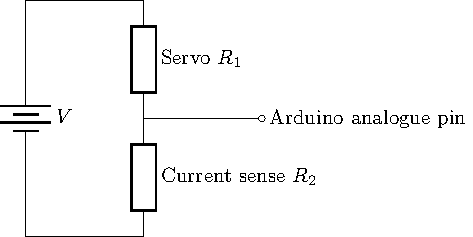
\includegraphics{current_measure_schematic/current_measure_schematic.pdf}
  \caption{Electrical diagram of current sensing.}
\end{figure}

The voltage measurement can be done by the Arduino by tapping off of the centre of the potential divider ($R_1$ and $R_2$).
The current sense resistor $R_2$ should be small so as to not affect the operation of the servo.
A value of $\SI{1}{\ohm}$ is sufficient for $R_2$.

\newpage
\subsection{Current smoothing}
The problem with measuring the current from a servo motor is it is driven by a pulse width modulation (PWM) signal.
For a torque controller to work it must receive a continuous value for the current.
Smoothing of the current signal can be achieved with a resistor capacitor (RC) circuit:
\begin{figure}[h]
  \centering
  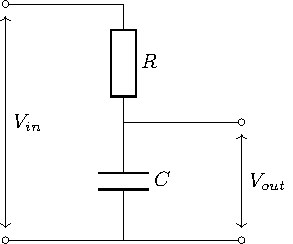
\includegraphics{rc_network_schematic/rc_network_schematic.pdf}
  \caption{Electrical diagram of RC network.}
\end{figure}

The current flow is:
\begin{equation}
    i(t) = \frac{V_{in}}{R}
    = \frac{V_R}{R}
    = C \frac{dV}{dt}
\end{equation}

Also, for $V_{out}$:
\begin{subequations}
  \begin{align}
    V_{out} &= V_C \\
    &= \frac{Q}{C} \\
    &= \frac{\int i(t)~dt}{C} \\
    &= \frac{1}{C} \int i(t)~dt \\
    &= \frac{1}{C} \int \frac{V_{in}}{R}~dt \\
    &= \frac{1}{RC} \int V_{in}~dt \\
    V_{out}(t) &= \frac{1}{RC} \int_0^t V_{in}~dt
  \end{align}
\end{subequations}

A pulse wave is a simple case of what the RC network will need to be able to smooth and can be defined as:
\begin{equation}
  f(x) =
  \begin{cases}
      5 & \text{if } x<T/2 \\
      0 & \text{if } x>T/2
  \end{cases}
\end{equation}

% Therefore for a $\SI{5}{\volt}$ input square wave:
% \begingroup
% \allowdisplaybreaks
% \begin{subequations}
%   \begin{align}
%     V_{out}(t) &= \frac{1}{RC} \int_0^t V_{in}~dt \\
%     &= \frac{1}{RC} \int_0^{nT} \begin{cases}
%         5 & \text{if } x<T/2 \\
%         0 & \text{if } x>T/2
%     \end{cases}~dt
%     \\
%     &= \frac{1}{RC}\sum_{n=0}^{n}\left[\int_n^{n+T/2} 5 ~dt + \int_{n+T/2}^{nT+T} 0 ~dt \right] \\
%     &= \frac{1}{RC}\sum_{n=0}^{n}\left[\int_n^{n+T/2} 5 ~dt \right] \\
%     &= \frac{1}{RC}\sum_{n=0}^{n}\left[5t \right]^{n+T/2}_n \\
%     &= \frac{1}{RC}\frac{5nT}{2} \\
%     &= \frac{5nT}{2RC}
%   \end{align}
% \end{subequations}
% \endgroup

To get the voltage across a capacitor charging start with Kirchhoff's voltage law:
\begin{equation}
    V_{in} = V_R + V_C
\end{equation}

For the current:
\begin{equation}
  i_R = i_C = C \frac{dV_C}{dt}
\end{equation}

So that:
\begin{equation}
    V_R = i_R R = i_C R = C \frac{dV_C}{dt} R
\end{equation}
\begin{subequations}
  \begin{align}
    V_{in} &= C \frac{dV_C}{dt} R + V_C \\
    RC\frac{dV_C}{dt} &= V_C - V_{in} \\
    \int \frac{1}{V_C - V_{in}} dV_C &= \int \frac{1}{RC} dt \\
    -\ln(V_{in} - V_C) &= \frac{t}{RC} + c \\
    V_{in} - V_C &= Ae^{-\frac{t}{RC}} \\
    V_{C,charge}(t) &= V_{in}\left[1-e^{-\frac{t}{RC}}\right]
  \end{align}
\end{subequations}

(Assuming $V_C(t=0)=0 \to A=V_{in}$).

Similarly for discharging:
\begin{subequations}
  \begin{align}
    V_{in} - V_C &= Ae^{-\frac{t}{RC}} \\
    0 - V_C &= Ae^{-\frac{t}{RC}} \\
    V_{C,discharge}(t) &= V_0\left[e^{-\frac{t}{RC}}\right]
  \end{align}
\end{subequations}

(Assuming $V_C(t=0)=V_0 \to A=-V_0$).

For response analysis of the RC circuit it makes sense to evaluate the circuit as a transfer function.
\begin{subequations}
  \begin{align}
    V_{in}(t) &= i(t) R + \frac{1}{C} \int i(t)~dt \\
    \mathcal{L}(V_{in}(t)) &= V_{in}(s) = I(s) R + \frac{1}{C}\frac{1}{s} I(s)
  \end{align}
\end{subequations}

\begin{subequations}
  \begin{align}
    V_{out}(t) &= \frac{1}{C} \int i(t)~dt \\
    \mathcal{L}(V_{in}(t)) &= V_{in}(s) = \frac{1}{C}\frac{1}{s} I(s)
  \end{align}
\end{subequations}

\begin{subequations}
  \begin{align}
  \frac{V_{out}(s)}{V_{in}(s)} &= \frac{\frac{1}{Cs} I(s)}{I(s)R + \frac{1}{Cs} I(s)} \\
  \frac{V_{out}(s)}{V_{in}(s)} &= \frac{\frac{1}{Cs}}{R+\frac{1}{Cs}} \\
  G(s) &= \frac{1}{RCs + 1}
  \end{align}
\end{subequations}

Similarly the pulse wave can be found as a transfer function:
\begin{subequations}
  \begin{align}
    \mathcal{L} &= \frac{1}{1-e^{-sT}} \int_0^T e^{-st} f(t)~dt \\
    &= \frac{1}{1-e^{-sT}} \int_0^{T/2} e^{-st} K~dt \\
    &= \frac{K}{1-e^{-sT}} \int_0^{T/2} e^{-st}~dt \\
    &= \frac{K}{1-e^{-sT}} \left[\frac{e^{-st}}{-s}\right]_0^{T/2} \\
    &= \frac{K}{(-s)(1-e^{-sT})} \left[e^{-st}\right]_0^{T/2} \\
    &= \frac{K}{(-s)(1-e^{-sT})} \left[e^{-Ts/2} - 1\right] \\
    &= \frac{K(e^{-Ts/2}-1)}{(-s)(1-e^{-sT})} \\
    &= \frac{K(1-e^{-Ts/2})}{(s)(1-e^{-sT})} \\
    &= \frac{K}{s}\frac{1-e^{-Ts/2}}{1-e^{-sT}}
  \end{align}
\end{subequations}

Combining the transfer functions:
\begin{subequations}
  \begin{align}
    &= \frac{Cs}{RCs + 1} \frac{K}{s} \frac{1-e^{-Ts/2}}{1-e^{-Ts}} \\
    &= \frac{KC}{s} \frac{s(1-e^{-Ts/2})}{(RCs + 1)(1-e^{-Ts})} \\
    &= \frac{KC(1-e^{-Ts/2})}{(RCs + 1)(1-e^{-Ts})}
  \end{align}
\end{subequations}

Using the final value theorem: $\lim\limits_{t\to \infty} f(t) = \lim\limits_{s\to 0} sF(s)$.
\begin{subequations}
  \begin{align}
    sF(s) &= s\frac{KC(1-e^{-Ts/2})}{(RCs + 1)(1-e^{-Ts})} \\
    &= \frac{sKC - sKCe^{-Ts/2}}{(RCs + 1)(1-e^{-Ts})} \\
    &= \frac{sKC - sKCe^{-Ts/2}}{RCs - RCse^{-Ts} + 1 - e^{-Ts}}
  \end{align}
\end{subequations}

% Given that $V_{out} = V_{C,charge}(t)-V_{C,discharge}(t)$:
% \begin{subequations}
%   \begin{align}
%     V_{out} &= V\left[1-e^{-\frac{T}{2RC}}\right] - V\left[e^{-\frac{T}{2RC}}\right] \\
%     V_{out} &= V\left[1-2e^{-\frac{T}{2RC}}\right]
%   \end{align}
% \end{subequations}
%-----------------------------------------------------------------------------%
\end{document}
%-----------------------------------------------------------------------------%
